\section{Технический проект}
\subsection{Компоненты приложения}
Компоненты приложения и взамодействия между ними можно увидеть на диаграмме компонентов, приведённой на рисунке ~\ref{components:image}.
\begin{figure}[h!]
	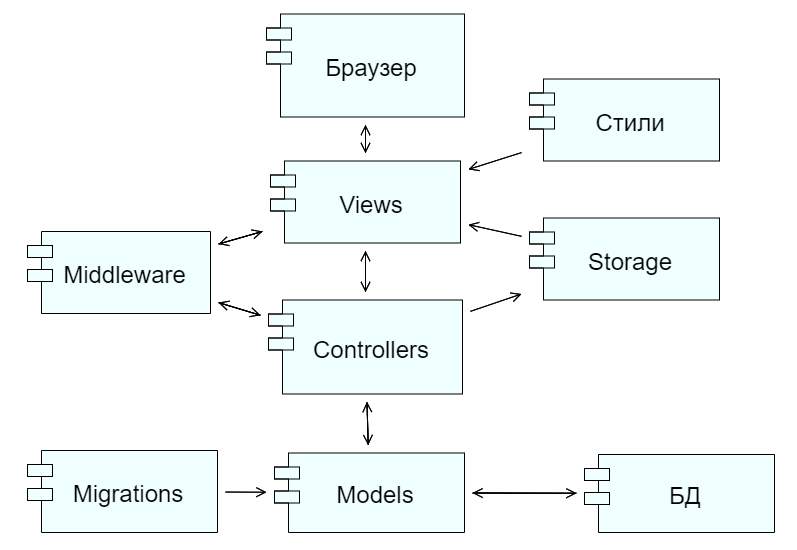
\includegraphics[width=0.8\linewidth]{components}
	\caption{Диаграмма компонентов приложения}
	\label{components:image}
\end{figure}
%\vspace{-\figureaboveskip} % двойной отступ не нужен (можно использовать, если раздел заканчивается картинкой)

\subsection{Обоснование выбора технологии проектирования}
\subsubsection{PHP}

PHP (Preprocessor Hypertext) — это язык программирования, который широко применяется для разработки веб-приложений и сайтов \cite{gizbert}. Он обладает рядом преимуществ, делающих его популярным среди разработчиков:
\begin{itemize}
	\item Простота изучения: PHP относительно легко понять и освоить, особенно если у пользователя уже есть базовые знания HTML. Это делает его привлекательным выбором для начинающих программистов.
	\item Широкая поддержка: PHP имеет большое сообщество разработчиков, которое обеспечивает широкую поддержку и доступ к множеству ресурсов для обучения и решения проблем.
	\item Гибкость: PHP позволяет легко интегрировать различные технологии, такие как базы данных, XML, JSON и другие веб-технологии.
	\item Оптимизация производительности: PHP предлагает множество инструментов для оптимизации производительности, включая кэширование, минификацию кода и многопоточность.
	\item Поддержка MVC (Model-View-Controller): PHP поддерживает архитектуру MVC, которая помогает организовать код и упрощает разработку и поддержку больших приложений.
	\item Интеграция с другими языками программирования: PHP может быть использован вместе с другими языками программирования, такими как JavaScript, Python и Ruby. Это позволяет разработчикам использовать лучшие практики и инструменты из разных языков.
	\item Поддержка фреймворков: Существует множество популярных PHP-фреймворков, таких как Laravel, Symfony, CodeIgniter и Yii, которые предоставляют дополнительные инструменты и структуры для ускорения разработки.
\end{itemize}

\subsubsection{MySQL}

MySQL - это одна из самых популярных систем управления базами данных (СУБД). Это программа, которая позволяет создавать и управлять базами данных реляционного типа с использованием языка стандартизированных запросов (SQL). MySQL отличается своей доступностью как по финансовой стороне, так и по уровню сложности. Она проста в управлении и имеет развитое сообщество пользователей \cite{brett}.

С практической точки зрения, система MySQL обладает рядом преимуществ:
\begin{itemize}
	\item высокая скорость работы благодаря отказу от некоторых стандартов языка;
	\item простая установка и интуитивно понятный интерфейс, что делает её доступной даже для новичков;
	\item отсутствие ограничений по количеству пользователей;
	\item гибкость за счёт открытого исходного кода;
	\item богатый выбор сторонних инструментов (плагинов), что позволяет настроить систему под конкретные потребности;
	\item поддержка больших таблиц, содержащих до 50 миллионов строк;
	\item высокий уровень безопасности;
	\item широкий функционал, который позволяет использовать систему в различных сферах.
\end{itemize}

Эта СУБД считается надежной и стабильной уже долгие годы. Она поддерживает разные виды таблиц, быстро выполняет команды и может быть модифицирована под индивидуальные нужды проекта.


\subsubsection{Blade}

При разработке представлений можно использовать PHP либо язык шаблонизатора Blade. Код представлений будет более чистым, если использовать Blade \cite{kirichenko}.

Преимущества Blade:
\begin{itemize}
	\item Простота использования. Для вывода данных достаточно использовать двойные фигурные скобки. Это позволяет избежать сложностей с выводом значений, экранированием строк и безопасностью.
	\item Безопасность. В отличие от PHP, где необходимо экранировать все выводимые данные, в Blade используются автоматические кавычки, что делает код более безопасным.
	\item Документированность. Blade хорошо документирован, что облегчает изучение и использование этого инструмента.
	\item Поддержка сообщества. Laravel имеет большое сообщество разработчиков, которые активно используют Blade и делятся своим опытом и решениями проблем.
	\item Расширяемость. Blade поддерживает пользовательские директивы, что позволяет расширять функциональность шаблонов без необходимости написания большого количества кода.
\end{itemize}

Выбор в пользу Blade добавляет дополнительный шаг в обработку шаблонов, т.к. все шаблоны Blade будут скомпилированы в PHP-код. Но благодаря кэшированию это не влияет на производительность приложения.

\subsection{Архитектура Laravel}
\subsubsection{Паттерн MVC}
Архитектура Laravel основана на шаблоне MVC (Model-View-Controller).
Это вариант архитектуры, при котором компоненты программы делятся на три части:
\begin{itemize}
	\item модель (model) предоставляет данные и методы работы с ними: запросы в базу данных, проверка на корректность;
	\item представление (view) показывает пользователю эти данные;
	\item контроллер (controller) направляет данные от пользователя к системе и наоборот.
\end{itemize}

Модель MVC предназначена для разделения логических частей приложения и создания их независимо друг от друга. 

\subsubsection{Жизненный цикл запроса}

Точкой входа всех запросов является файл public/index.php. Он загружает сгенерированное Composer определение автозагрузчика и извлекает экземпляр приложения Laravel из файла bootstrap/app.php.

В зависимости от типа запроса, он отправляется либо в ядро HTTP, либо в ядро Console.

Ядро HTTP находится в файле app/Http/Kernel.php и расширяет класс Illuminate/Foundation/Http/Kernel. Оно определяет массив bootstrappers — загрузчиков, которые будут выполняться перед обработкой запроса. Эти загрузчики настраивают обработку ошибок, настраивают логи, определяют окружение приложения и выполняют другие задачи, которые необходимо выполнить перед фактической обработкой запроса.

Ядро HTTP также определяет список HTTP-middleware, через которые должны пройти все запросы, прежде чем они будут переданы приложению. Эти middleware обрабатывают чтение и запись HTTP-сессии, определяют, находится ли приложение в режиме обслуживания, проверяют CSRF-токены и многое другое.

Одним из наиболее важных действий по начальной загрузке ядра является загрузка сервис-провайдеров — поставщиков услуг приложения. Сервис-провайдеры несут ответственность за начальную загрузку различных компонентов фреймворка, таких как базы данных, очереди, компоненты валидации и маршрутизации. Все сервис-провайдеры приложения настраиваются в массиве providers файла config/app.php.

После создания экземпляров провайдеров для них будет вызываться метод register. Как только все провайдеры будут зарегистрированы, для каждого из них будет вызван метод boot. Метод boot() в Laravel используется для определения кода, который должен быть выполнен при регистрации поставщика услуг. Этот метод обычно используется для регистрации пользовательских привязок, конфигураций и слушателей событий.

Одним из наиболее важных сервис-провайдеров в Laravel-приложении является App/Providers/RouteServiceProvider. Этот сервис-провайдер загружает файлы маршрутов, содержащиеся в каталоге routes.

После загрузки приложения и регистрации всех сервис-провайдеров запрос будет передан для обработки маршрутизатору. Маршрутизатор отправит запрос в маршрут или контроллер, а также запустит указанное middleware для данного маршрута. Если запрос проходит через все middleware соответствующего маршрута, будет выполнен метод маршрута или контроллера, а ответ, возвращённый методом маршрута или контроллера, будет отправлен обратно через цепочку middleware, давая приложению возможность изменить или проверить исходящий ответ.

Когда ответ возвращается через middleware, метод handle ядра HTTP возвращает объект ответа, а файл index.php вызывает метод send, который отправляет содержимое ответа в веб-браузер пользователя.


\subsubsection{Сервис-провайдеры}

Сервис-провайдеры являются центральным местом начальной загрузки всех возможностей Laravel. Под загрузкой подразумевается регистрация нужных сервисов, включая регистрацию привязок к служебному контейнеру, прослушивателей событий, middleware и даже маршрутов.

Все классы сервис-провайдеров хранятся в config/app.php. Провайдеры, имеющиеся там изначально, загружают основные компоненты Laravel, такие как почтовый рассыльщик, очередь, кэш и другие. Многие из этих классов провайдеров являются «отложенными». Это означает, что они будут загружаться не при каждом запросе, а только при необходимости предоставляемых ими услуг. Пользователь может создавать собственные сервис-провайдеры для своего приложения.

Все сервис-провайдеры расширяют класс Illuminate/Support/ServiceProvider. Класс провайдера содержит 2 метода — register и boot. Метод register предназначен для привязки к сервисному контейнеру. Внутри любого из методов класса-провайдера всегда доступно свойство \$app, которое предоставляет доступ к сервисному контейнеру. Метод boot используется для расширения возможностей фреймворка, например, для создания новых blade-директив и запускается только после выполнения всех методов register.

\subsubsection{Сервис-контейнеры}

Сервис-контейнер или контейнер служб – это инструмент для управления зависимостями классов и выполнения внедрения зависимостей. Зависимости классов «вводятся» в класс через конструктор в виде аргументов или, в некоторых случаях, через методы-сеттеры. При создании класса или вызове методов фреймворк смотрит на список аргументов и, если нужно, создаёт экземпляры необходимых классов и сам подаёт их на вход конструктора или метода. 

Все контроллеры регистрируются через сервис-контейнер, поэтому при получении класса контроллера из контейнера автоматически получаются все зависимости, указанные в аргументах конструктора и других методах контроллера.


\subsubsection{Фасады}

Фасады предоставляют «статический» интерфейс для классов, доступных в сервис-контейнере приложения. Все фасады Laravel расширяют базовый класс Illuminate/Support/Facades/Facade. Базовый класс Facade использует магический метод \_\_callStatic(), чтобы делегировать вызовы из фасада объекту, извлеченному из контейнера.

Фасады предоставляют краткий и понятный синтаксис, который позволяет пользоваться функциями laravel без запоминания длинных названий классов, которые должны внедряться вручную. В дополнении к фасадам, Laravel предлагает множество глобальных вспомогательных функций, которые упрощают взаимодействие с общими функциями Laravel. Они доступны глобально и не требуют импортирования каких-либо классов для их использования. Многие вспомогательные функции выполняют те же задачи, что и соответствующие фасады.


\subsection{Структура каталогов}

Структура каталогов приложения включает следующие основные каталоги:
\begin{enumerate}
	\item App — содержит подкаталоги Console, Exceptions, Http, Models и Providers. Каталог Console содержит пользовательские команды Artisan. Каталог Exceptions содержит обработчик исключений. Каталог Http содержит контроллеры, middleware и запросы форм. Каталог Models содержит классы моделей Eloquent. Каталог Providers содержит сервис провайдеры, подготавливающие приложение к входящим запросам.
	\item Bootstrap — содержит файл app.php, загружающий фреймворк. Также в папке bootstrap находится папка cache, которая содержит сгенерированные фреймворком файлы для оптимизации производительности, например, кэш-файлы маршрутов и сервисов.
	\item Config — содержит файлы конфигурации приложения.
	\item Database — содержит миграции базы данных, фабрики моделей и данные для заполнения.
	\item Public — содержит index.php, являющийся точкой входа для всех запросов, поступающих в приложение, и ссылку на storage.
	\item Resources — содержит представления (view).
	\item Routes — содержит все определения маршрутов для приложения.
	\item Storage — разделён на подкаталоги storage/app, storage/framework и storage/logs. Каталог storage/framework используется для хранения кэшей. Storage/log хранит файлы журналов (логи) приложения. В каталоге storage/app/public хранятся изображения товаров.
	\item Tests — содержит автоматические тесты.
	\item Vendor — хранит зависимости, установленные через менеджер пакетов Composer. 
\end{enumerate}

\subsection{Структура базы данных}

В таблице \ref{bd:table} показана структура таблицы plant\_categories.

\begin{xltabular}{\textwidth}{|c|X|X|X|}
	\caption{\label{bd:table}Таблица plant\_categories} \\ \hline
	\thead {Тип ключа} & \thead {Обязательность} & \thead {Имя столбца}
	& \thead {Тип данных} \\ \hline
	\endfirsthead
	\continuecaption{Продолжение таблицы \ref{bd:table}}
	\thead {Тип ключа} & \thead {Обязательность} & \thead {Имя столбца}
	& \thead {Тип данных} \\ \hline
	\finishhead
	primary key & да & id & integer \\ \hline 
	~ & да &	name & string \\ \hline 
	~ & да &	description & text
\end{xltabular}


В таблице \ref{bd2:table} показана структура таблицы plant\_genera.

\begin{xltabular}{\textwidth}{|c|X|X|X|}
	\caption{Таблица plant\_genera\label{bd2:table}}\\ \hline
	\thead {Тип ключа} & \thead {Обязательность} & \thead {Имя столбца}
	& \thead {Тип данных} \\ \hline
	\endfirsthead
	\continuecaption{Продолжение таблицы \ref{bd2:table}}
	\thead {Тип ключа} & \thead {Обязательность} & \thead {Имя столбца}
	& \thead {Тип данных} \\ \hline
	\finishhead
	primary key & да & name & string \\ \hline 
	~ & да & description & text
\end{xltabular}

В таблице \ref{bd3:table} показана структура таблицы product\_types.

\begin{xltabular}{\textwidth}{|c|X|X|X|}
	\caption{Таблица product\_types\label{bd3:table}}\\ \hline
	\thead {Тип ключа} & \thead {Обязательность} & \thead {Имя столбца}
	& \thead {Тип данных} \\ \hline
	\endfirsthead
	\continuecaption{Продолжение таблицы \ref{bd3:table}}
	\thead {Тип ключа} & \thead {Обязательность} & \thead {Имя столбца}
	& \thead {Тип данных} \\ \hline
	\finishhead
	primary key & да & name & string
\end{xltabular}

В таблице \ref{bd4:table} показана структура таблицы plant\_colors.

\begin{xltabular}{\textwidth}{|c|X|X|X|}
	\caption{Таблица plant\_colors\label{bd4:table}}\\ \hline
	\thead {Тип ключа} & \thead {Обязательность} & \thead {Имя столбца}
	& \thead {Тип данных} \\ \hline
	\endfirsthead
	\continuecaption{Продолжение таблицы \ref{bd4:table}}
	\thead {Тип ключа} & \thead {Обязательность} & \thead {Имя столбца}
	& \thead {Тип данных} \\ \hline
	\finishhead
	primary key & да & name & string
\end{xltabular}

В таблице \ref{bd5:table} показана структура таблицы climate\_zones.

\begin{xltabular}{\textwidth}{|c|X|X|X|}
	\caption{Таблица climate\_zones\label{bd5:table}}\\ \hline
	\thead {Тип ключа} & \thead {Обязательность} & \thead {Имя столбца}
	& \thead {Тип данных} \\ \hline
	\endfirsthead
	\continuecaption{Продолжение таблицы \ref{bd5:table}}
	\thead {Тип ключа} & \thead {Обязательность} & \thead {Имя столбца}
	& \thead {Тип данных} \\ \hline
	\finishhead
	primary key & да & zone\_number & integer \\ \hline 
	~ & да & lower\_temp\_limit & integer \\ \hline 
	~ & да & upper\_temp\_limit & integer
\end{xltabular}

В таблице \ref{bd6:table} показана структура таблицы light\_modes.

\begin{xltabular}{\textwidth}{|c|X|X|X|}
	\caption{Таблица light\_modes\label{bd6:table}}\\ \hline
	\thead {Тип ключа} & \thead {Обязательность} & \thead {Имя столбца}
	& \thead {Тип данных} \\ \hline
	\endfirsthead
	\continuecaption{Продолжение таблицы \ref{bd6:table}}
	\thead {Тип ключа} & \thead {Обязательность} & \thead {Имя столбца}
	& \thead {Тип данных} \\ \hline
	\finishhead
	primary key & да & name & string
\end{xltabular}

В таблице \ref{bd7:table} показана структура таблицы soils.

\begin{xltabular}{\textwidth}{|c|X|X|X|}
	\caption{Таблица soils\label{bd7:table}}\\ \hline
	\thead {Тип ключа} & \thead {Обязательность} & \thead {Имя столбца}
	& \thead {Тип данных} \\ \hline
	\endfirsthead
	\continuecaption{Продолжение таблицы \ref{bd7:table}}
	\thead {Тип ключа} & \thead {Обязательность} & \thead {Имя столбца}
	& \thead {Тип данных} \\ \hline
	\finishhead
	primary key & да & name & string
\end{xltabular}

В таблице \ref{bd8:table} показана структура таблицы life\_cycles.

\begin{xltabular}{\textwidth}{|c|X|X|X|}
	\caption{Таблица life\_cycles\label{bd8:table}}\\ \hline
	\thead {Тип ключа} & \thead {Обязательность} & \thead {Имя столбца}
	& \thead {Тип данных} \\ \hline
	\endfirsthead
	\continuecaption{Продолжение таблицы \ref{bd8:table}}
	\thead {Тип ключа} & \thead {Обязательность} & \thead {Имя столбца}
	& \thead {Тип данных} \\ \hline
	\finishhead
	primary key & да & name & string
\end{xltabular}

В таблице \ref{bd9:table} показана структура таблицы plants.

\begin{xltabular}{\textwidth}{|c|X|X|X|}
	\caption{Таблица plants\label{bd9:table}}\\ \hline
	\thead {Тип ключа} & \thead {Обязательность} & \thead {Имя столбца}
	& \thead {Тип данных} \\ \hline
	\endfirsthead
	\continuecaption{Продолжение таблицы \ref{bd9:table}}
	\thead {Тип ключа} & \thead {Обязательность} & \thead {Имя столбца}
	& \thead {Тип данных} \\ \hline
	\finishhead
	primary key & да & id & integer \\ \hline
	~ & да & name & string \\ \hline
	~ & да & description & text \\ \hline
	~ & да & quantity & integer \\ \hline
	~ & да & price & decimal \\ \hline
	~ & нет & image & text \\ \hline
	~ & да & flower\_diameter & decimal \\ \hline
	foreign key & да & genus & string \\ \hline
	foreign key & да & product\_type & string \\ \hline
	foreign key & да & life\_cycle & string \\ \hline
	foreign key & да & soil & string \\ \hline
	foreign key & да & landing\_place & string \\ \hline
	foreign key & да & climate\_zone & integer \\ \hline
	foreign key & да & flower\_color1 & string \\ \hline
	foreign key & нет & flower\_color2 & string \\ \hline
	foreign key & нет & flower\_color3 & string \\ \hline
	foreign key & да & leaf\_color1 & string \\ \hline
	foreign key & нет & leaf\_color2 & string \\ \hline
	foreign key & нет & leaf\_color3 & string
\end{xltabular}

В таблице \ref{bd10:table} показана структура таблицы users.

\begin{xltabular}{\textwidth}{|c|X|X|X|}
	\caption{Таблица users\label{bd10:table}}\\ \hline
	\thead {Тип ключа} & \thead {Обязательность} & \thead {Имя столбца}
	& \thead {Тип данных} \\ \hline
	\endfirsthead
	\continuecaption{Продолжение таблицы \ref{bd10:table}}
	\thead {Тип ключа} & \thead {Обязательность} & \thead {Имя столбца}
	& \thead {Тип данных} \\ \hline
	\finishhead
	primary key & да & id & integer \\ \hline
	~ & да & name & string \\ \hline
	~ & да & email & string \\ \hline
	~ & нет & email\_verified\_at & timestamp \\ \hline
	~ & да & password & string \\ \hline
	~ & да & is\_admin & tinyInteger
\end{xltabular}

В таблице \ref{bd11:table} показана структура таблицы orders.

\begin{xltabular}{\textwidth}{|c|X|X|X|}
	\caption{Таблица orders\label{bd11:table}}\\ \hline
	\thead {Тип ключа} & \thead {Обязательность} & \thead {Имя столбца}
	& \thead {Тип данных} \\ \hline
	\endfirsthead
	\continuecaption{Продолжение таблицы \ref{bd11:table}}
	\thead {Тип ключа} & \thead {Обязательность} & \thead {Имя столбца}
	& \thead {Тип данных} \\ \hline
	\finishhead
	primary key & да & id & integer \\ \hline
	~ & да & status & integer \\ \hline
	~ & нет & name & text \\ \hline
	~ & нет & phone & text \\ \hline
	~ & нет & address & text \\ \hline
	~ & нет & email & string \\ \hline
	foreign key & нет & user\_id & integer
\end{xltabular}

В таблице \ref{bd12:table} показана структура таблицы order\_plant.

\begin{xltabular}{\textwidth}{|c|X|X|X|}
	\caption{Таблица order\_plant\label{bd12:table}}\\ \hline
	\thead {Тип ключа} & \thead {Обязательность} & \thead {Имя столбца}
	& \thead {Тип данных} \\ \hline
	\endfirsthead
	\continuecaption{Продолжение таблицы \ref{bd12:table}}
	\thead {Тип ключа} & \thead {Обязательность} & \thead {Имя столбца}
	& \thead {Тип данных} \\ \hline
	\finishhead
	primary key & да & id & integer \\ \hline
	~ & да & plant\_count & integer \\ \hline
	foreign key & да & order\_id  & integer \\ \hline
	foreign key & да & plant\_id & integer
\end{xltabular}

В таблице \ref{bd13:table} показана структура таблицы plant\_plant\_category.

\begin{xltabular}{\textwidth}{|c|X|X|X|}
	\caption{Таблица plant\_plant\_category\label{bd13:table}}\\ \hline
	\thead {Тип ключа} & \thead {Обязательность} & \thead {Имя столбца}
	& \thead {Тип данных} \\ \hline
	\endfirsthead
	\continuecaption{Продолжение таблицы \ref{bd13:table}}
	\thead {Тип ключа} & \thead {Обязательность} & \thead {Имя столбца}
	& \thead {Тип данных} \\ \hline
	\finishhead
	primary key & да & id & integer \\ \hline
	foreign key & да & plant\_category\_id   & integer \\ \hline
	foreign key & да & plant\_id & integer
\end{xltabular}

\subsection{Список контроллеров}

Каталог Controller содержит следующие контроллеры: 
\begin{itemize}
	\item Controller – родительский контроллер для остальных контроллеров;
	\item MainController – отвечает за отображение некоторых страниц, в том числе главной страницы сайта;
	\item HomeController – отвечает за отображение заказов пользователя;
	\item BasketController – отвечает за добавление товара в корзину и отображение корзины.
\end{itemize}

Каталог Controller также содержит подкаталоги Admin и Auth.

\subsubsection{Контроллеры подкаталога Admin}
Подкаталог Admin предназначен для контроллеров, предоставляющих методы для администратора сайта:
\begin{itemize}
	\item CategoryController – ресурсный контроллер для управления категориями;
	\item OrderController – отвечает за отображение заказов у администратора;
	\item PlantController – ресурсный контроллер для управления товарами.
\end{itemize}

\subsubsection{Контроллеры подкаталога Auth}
Подкаталог Auth объединяет контроллеры для регистрации и авторизации: 
\begin{itemize}
	\item ConfirmPasswordController – предназначен для обработки подтверждения пароля;
	\item ForgotPasswordController – отвечает за отправку электронных писем для сброса пароля;
	\item LoginController – обрабатывает аутентификацию ;
	\item RegisterController – обрабатывает регистрацию новых пользователей;
	\item ResetPasswordController – содержит логику сброса пароля;
	\item VerificationController – отвечает за переход пользователей на другую страницу после верификации.
\end{itemize}

\subsection{Список представлений}

Каталог views содержит подкаталоги frontend, orders, auth, layouts и admin.

\subsubsection{Представления подкаталога frontend}
Подкаталог frontend содержит страницы для просмотра и заказа товаров:
\begin{itemize}
	\item index.blade.php – главная страница со всеми товарами;
	\item categories.blade.php – страница категорий товаров;
	\item category.blade.php – страница категории;
	\item product.blade.php – страница товара;
	\item basket.blade.php – корзина;
	\item order.blade.php – страница оформления заказа;
\end{itemize}

\subsubsection{Представления подкаталога orders}
Подкаталог orders содержит страницы заказов пользователя:
\begin{itemize}
	\item home.blade.php – страница заказов;
	\item order.blade.php – страница заказа.
\end{itemize}

\subsubsection{Представления подкаталога auth}
Подкаталог auth содержит страницы авторизации и регистрации:
\begin{itemize}
	\item login.blade.php – страница аутентификации;
	\item register.blade.php – страница регистрации;
	\item verify.blade.php – страница верификации;
\end{itemize}

В этом подкаталоге также есть раздел passwords, объединяющий страницы для пароля:
\begin{itemize}
	\item confirm.blade.php – форма для подтверждения пароля;
	\item email.blade.php – форма для ввода адреса электронной почты для сброса пароля;
	\item reset.blade.php – форма для создания нового пароля.
\end{itemize}

\subsubsection{Представления подкаталога layouts}
Подкаталог layouts содержит представления, используемые другими представлениями:
\begin{itemize}
	\item master.blade.php – HTML-каркас для других представлений с подключёнными стилями и меню;
	\item card.blade.php – шаблон карточки товара;
	\item filters.blade.php – поле выбора характеристик, по которым можно отфильтровать товары.
\end{itemize}

\subsubsection{Представления подкаталога admin}
Подкаталог admin делится на разделы categories, orders и plants. 

Раздел categories содержит страницы для работы с категориями:
\begin{itemize}
	\item index.blade.php – страница категорий;
	\item show.blade.php – страница категории;
	\item form.blade.php – страница добавления или редактирования категории.
\end{itemize}

Раздел orders содержит страницы для просмотра заказов:
\begin{itemize}
	\item index.blade.php – страница заказов;
	\item show.blade.php – страница заказа;
\end{itemize}

Раздел plants содержит страницы для работы с товарами:
\begin{itemize}
	\item index.blade.php – страница товаров;
	\item show.blade.php – страница товара;
	\item form.blade.php – страница добавления или редактирования товара.
\end{itemize}

\subsection{Стили приложения}
Стили приложения можно найти по пути public/assets/css. Они представлены двумя файлами: bootstrap.min.css и starter-template.css. Эти стили подключаются в представлении layouts/master.blade.php. Файл bootstrap.min.css позволяет использовать возможности фреймворка Bootstrap для стилизации контента с помощью отдельных классов и компонентов. Одна из ключевых особенностей фреймворка – использование сетки, которая позволяет легко управлять распределением контента на разных размерах экранов.
